\documentclass[a4paper]{article}

\usepackage{CJK}
\usepackage{amsthm}
\usepackage{tikz}

\theoremstyle{definition}
\newtheorem{lemma}{Lemma}

\title{Report for EI339 Artificial Intelligence: Homework 4}
\author{517030910384 徐尚宁}
\date{}

\begin{document}

\begin{CJK}{UTF8}{gbsn}
    \maketitle
\end{CJK}

\section*{Q1}

Only when the white piece is adjacent to the black at the start can A win the
game.

\begin{proof}
    When the white and the black piece are adjacent to each other. A can simply
    move its piece to eat their opponent.

    We claim that if A is about to move and the $L_1$ distance between the white
    and black piece $d \geq 2$, then A will lose the game, which basically means
    that A will lose as long as the white piece is not adjacent to the black at
    the start.

    We propose the following strategy for B that leads to B's victory when $d
    \geq 2$.
    \begin{enumerate}
        \item For $d = 2$ and it is A's turn to move, there are two cases:
        \begin{itemize}
            \item If the black and the white piece form a straight line, no
            matter how the white moves, B just moves the black piece along the
            line one grid at a time.
            \item If the black is diagonally adjacent to the white, then B just
            imitates A's last move.
        \end{itemize}
        \item For $d > 2$, and it is A's turn to move, there are two cases:
        \begin{itemize}
            \item If the white moves away from the black, then B chooses a
            direction in which moving two grids will decrease $d$ by 2.
            \item If the white moves towards the black, and after the move, it
            is B's turn,
            \begin{itemize}
                \item If $d = 2$, either the black can simply eat the white when
                they are on a straight line, or when they diagonally adjacent to
                each other, the black piece moves two grids in a direction such
                that before and after the move, $d$ doesn't change.
                \item If $d = 3$, there must exist a direction in which the
                black moves one grid and decreases $d$ by one.
            \end{itemize}
        \end{itemize}
    \end{enumerate}

    The full proof follows below.

    When $d = 2$, there are two states for the chessboard: either the two pieces
    form a straight line, or the white is adjacent to the black diagonally. A
    can't move its piece towards the black piece (that is, choose a move that
    decreases the $L_1$ distance), because doing so in either case will allow
    the black piece to directly eat the white. Suppose that the two pieces are
    on a chessboard without boundary. For the white piece to survive, A will
    move it away from the black. We give a strategy for B on how to move with
    regard to each of the two cases.

    In the former case, the white and black form a straight line. No matter how
    A moves, B just needs to move its piece along the straight line for one step
    towards the white. If A's move was along the line, B's move will keep the
    two pieces in the same relative position. Or if A moved its piece
    perpendicular to the line, B's move will make the black piece diagonally
    adjacent to the white, which transforms this case into the latter case.

    In the latter case, B needs to imitate A's move to maintain their relative
    position. If the chessboard has no boundary, the strategy described above
    essentially leads to a draw, but the chessboard size is finite. The black
    piece will at some point encounter the boundary and, if the black and white
    are on a straight line, the black are forced to move sideways, leading to
    the former case.

    The game concludes when the white piece has no way to retreat.

    If B wins the game for $2 \leq d \leq k$, we want to prove that B still wins
    for $d \leq k + 1$. For $d = k + 1$, there are two possibilities for A's
    move: A can move the white piece towards or away from the black piece.
    \begin{itemize}
        \item If the white piece moves away from the black piece, then after A's
        move, $d = k + 2 \geq 4$ because $k \geq 2$. In this case, there must
        exist a direction in which the black piece can move 2 grids to decrease
        $d$ by 2 to $k$. Consider the rectangle formed by the white and black
        piece as its two opposite corners. Such rectangle must have one side
        whose length is greater than 2 because the rectangle's perimeter is
        equal to $d = k$. B moves its piece in such direction and then it is A's
        turn and $d = k$, so B wins.
        \item If the white piece moves towards the black piece, then $d = k$
        after A's move. If $k \geq 4$, B can still apply the strategy above
        because after such move, $d = k - 2 \geq 2$ and B wins.

        If, after A's move, $k < 4$, we have to separately discuss the cases for
        $k = 2$ or 3. If $k = 3$, B just moves its piece one grid towards the
        white piece so that at A's turn $d = 2$ and B wins. If $k = 2$, B will
        make a decision based on the state of the chessboard. If the black and
        white forms a straight line, the black piece can directly eats the
        white. If the black is adjacent to the white diagonally, there must
        exist a direction in which the white piece can move two grids such that
        before and after the move the $L_1$ distance $d$ doesn't change. Because
        after B's move, $d = 2$ and now it is A's turn, so B wins.

        There is one case where such move is impossible, that is when the white
        piece is at the corner, the black piece is diagonally adjacent to it and
        it is B's turn. We argue that this scenario can't happen under the
        assumption that A and B are rational. Because now it is B's turn, let
        this turn be the $i$th turn and consider what is A's move in turn $i -
        1$. Because the white piece can only move one grid at a time, the black
        would have been adjacent to the white at turn $i - 1$. A should have
        already won at turn $i - 1$ because the white can eat the black, and
        since B is rational, they would not have moved the black piece next to
        the white.
    \end{itemize}
    With the complete strategy for B outlined above, we conclude that A will
    only win when $d = 1$.
\end{proof}

\section*{Q2}

\begin{figure}[ht]
    \centering
    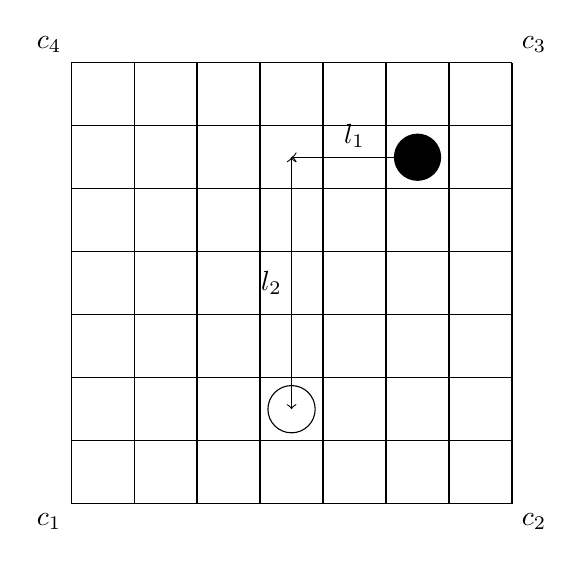
\begin{tikzpicture}
        \draw[step=0.8cm] (0, 0) grid (5.6, 5.6);
        \draw (2.8, 1.2) circle [radius=0.3cm];
        \fill (4.4, 4.4) circle [radius=0.3cm];
        \draw (0, 0) node [anchor=north east] {$c_1$};
        \draw (5.6, 0) node [anchor=north west] {$c_2$};
        \draw (5.6, 5.6) node [anchor=south west] {$c_3$};
        \draw (0, 5.6) node [anchor=south east] {$c_4$};
        \draw [<->] (2.8, 4.4) -- node [above] {$l_1$} (4.4, 4.4);
        \draw [<->] (2.8, 1.2) -- node [left] {$l_2$} (2.8, 4.4);
    \end{tikzpicture}
    \caption{Illustration for Q2's proof.}
    \label{fig:q2-proof-illustration}
\end{figure}

\begin{proof}
    We impose a left-hand coordinate system on the chessboard, with the origin
    at the lower left corner $c_1$. Similar to the proof in Q1, we give an
    strategy for B to bound the total number of rounds from above. Consider
    again the rectangle formed by the two pieces as its opposite corners, like
    the rectangle bounded by two sides $l_1$ and $l_2$ in
    Figure~\ref{fig:q2-proof-illustration}. Our strategy for B is that the black
    piece should walk two grids along the direction of the longer side of the
    rectangle i.e. $l_2$, until either
    \begin{enumerate}
        \item it is B's turn and walking two grids this turn will make the two
        pieces form a $2 \times 1$ rectangle. In this case, the black piece
        should walks one grid along the side with length 2, making the rectangle
        a square.
        \item Or, walking one grid at B's turn can make $l_1 = l_2$. The black
        piece should walk one grid at that turn.
        \item Or, the rectangle formed by the two pieces is now a square. After
        this point, the black piece will force the white piece into a corner,
        walking one or two grids at a time.
    \end{enumerate}

    Our strategy is termed as ``maintain the square'', that is, B seeks to make
    the rectangle a square as quickly as possible and maintain the square until
    the white piece is cornered. In the rest of the proof, we explain how the
    strategy gives an upper bound of $4n$.

    Consider the example given in Figure~\ref{fig:q2-proof-illustration}, where
    $l_1 < l_2$. We term the corners $c_3$ and $c_4$ as the \emph{impossible}
    corners because at the game's start, A realizes that it cannot reach $c_3$
    and $c_4$ in any means. By contrast, $c_1$ and $c_2$ are the \emph{possible}
    corners to which the white piece may retreat.

    Our strategy gives the following guarantee:
    \begin{lemma}
        Before $l_1 = l_2$, the black piece only walks in one direction.
    \end{lemma}

    Once $l_1 = l_2$, there is only one corner to which the white piece may
    retreat. The rectangle formed by that corner and the black piece as its
    opposite corners will \emph{cover} the white piece, and the white piece will
    never be able to escape this rectangle, because the black piece always walks
    faster. The strategy for B after $l_1 = l_2$ is quite flexible as it can
    move the piece one or two grids, but as it has been proved in Q1, B will
    win.

    The key idea of this strategy is that the black piece is essentially moving
    into a corner from its start position, no matter how A moves. For the black
    piece to move into a corner, we need at most $2n$ rounds for B, and at the
    same time $2n$ rounds for A, so the total number of rounds $K \leq 4n$.
\end{proof}

\end{document}
